\section{映射}
\subsection{映射的概念}
\begin{defn}{映射定义}{}
    设$X,Y$是两个\textcolor{red}{非空集合},如果\textbf{存在}一个\textcolor{red}{法则$f$},使得对$X$中\textbf{每个元素}$x$,按法则$f$,在$Y$中有\textbf{唯一确定的元素}$y$与之对应,那么称$f$为从$X$到$Y$的映射,记作
    $$
        f:X \to Y
    $$
    其中$y$称为元素$x$(在映射$f$下)的像,并记住$f(x)$,即
    $$
        y=f(x)
    $$
    而元素$x$称为元素$y$(在映射$f$下)对一个原像;
\end{defn}
需要注意的是,从映射的概念可以看出,映射法则$f$可以有多个,但是只要有一个满足即可.
\subsection{逆映射和复合映射}
\begin{defn}{逆映射的定义}{}
    设$f$是$X$到$Y$的单射,则由定义,对每个$y \in R_f$,有唯一的$x \in X$,适合$f(x)=y$,于是,我们可定义一个从$R_f$到$X$的新映射$g$,即
    \begin{center}
        $g: R_f \to X$
    \end{center}
    对每个$y \in R_f$,规定$g(y)=x$,这个$x$满足$f(x)=y$.这个映射$g$称为$f$的逆映射,记作$f^{-1}$,其定义域为$D_{f^{-1}}=R_f$,值域$R_{f^{-1}}=X$.根据上述定义可知,只有单射才存在逆映射.
\end{defn}
\begin{defn}{复合映射的定义}{}
    设有两个映射
    \begin{center}
        $g: X \to Y_1$ \qquad $f:Y_2 \to Z$
    \end{center}
    其中$Y_1 \subset Y_2$,则由映射$g$和$f$可以定出一个从$X$到$Z$的对应法则,它将每个$x \in X$映成$f[g(x)] \in Z$.显然,这个对应法则确定了一个从$X$到$Z$的映射,这个映射称为映射$g$和$f$构成的复合映射,记作$f \circ g$,即
    $$
        f\circ g:X\to Z,(f\circ g)(x)=f[g(x)],x\in X.
    $$
    由复合映射的定义可知,映射$g$和$f$构成复合映射的条件是:$g$的值域$R_g$,必须包含在$f$的定义域内,即$R_g \subset D_f$.否则,不能构成复合映射.由此可以知道,映射$g$和$f$复合是有顺序的.
\end{defn}
\subsection{映射的分类}
\begin{itemize}
    \item 设$f$是从集合$X$到集合$Y$的映射,若$R_f=Y$,即$Y$中任一元素$y$都是$X$中某元素的像,则称$f$为$X$到$Y$上的\uwave{映射或满射};
    \item 若对$X$中任意两个不同元素$x_1 \neq x_2$,它们的像$f(x_1) \neq f(x_2)$,则称$f$为$X$到$Y$的\uwave{单射};
    \item 若映射$f$既是单射,又是满射,则称$f$为\uwave{一一映射(或双射)}
\end{itemize}
\begin{criterion}{单值函数与多值函数}{}
    事实上上述定义的函数为\textbf{单值函数},若给定一个$x_1$,对应一个$y_1$。给另外一个$x_2$,对应另外一个$y_2$,即\textbf{“一对一”}.其图像如下图所示\\
    \tikzset{every picture/.style={line width=0.55pt}} %set default line width to 0.75pt        
    \begin{center}
        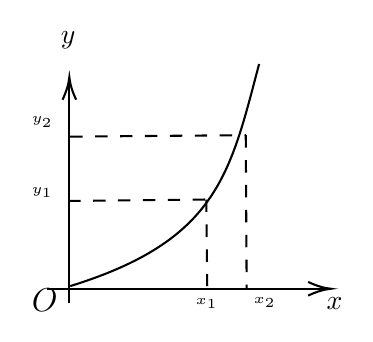
\begin{tikzpicture}[x=0.75pt,y=0.75pt,yscale=-1,xscale=1]
            %uncomment if require: \path (0,300); %set diagram left start at 0, and has height of 300
            %Straight Lines [id:da7957062642323978] 
            \draw    (220.57,170.29) -- (355.57,170.29) ;
            \draw [shift={(357.57,170.29)}, rotate = 180] [color={rgb, 255:red, 0; green, 0; blue, 0 }  ][line width=0.75]    (10.93,-3.29) .. controls (6.95,-1.4) and (3.31,-0.3) .. (0,0) .. controls (3.31,0.3) and (6.95,1.4) .. (10.93,3.29)   ;
            %Straight Lines [id:da31198976122474575] 
            \draw    (231.57,177.29) -- (231.57,70.29) ;
            \draw [shift={(231.57,68.29)}, rotate = 90] [color={rgb, 255:red, 0; green, 0; blue, 0 }  ][line width=0.75]    (10.93,-3.29) .. controls (6.95,-1.4) and (3.31,-0.3) .. (0,0) .. controls (3.31,0.3) and (6.95,1.4) .. (10.93,3.29)   ;
            %Straight Lines [id:da5655592463420158] 
            \draw  [dash pattern={on 4.5pt off 4.5pt}]  (297.57,127.29) -- (298,169) ;
            %Straight Lines [id:da8571495896140271] 
            \draw  [dash pattern={on 4.5pt off 4.5pt}]  (316.57,96.29) -- (317,170) ;
            %Straight Lines [id:da505677150137505] 
            \draw  [dash pattern={on 4.5pt off 4.5pt}]  (232,97) -- (316.57,96.29) ;
            %Straight Lines [id:da9798041145850536] 
            \draw  [dash pattern={on 4.5pt off 4.5pt}]  (231,128) -- (297.57,127.29) ;
            %Curve Lines [id:da5109656726245018] 
            \draw    (232,169) .. controls (303,147) and (309,115) .. (323,62) ;
            % Text Node
            \draw (226,45) node [anchor=north west][inner sep=0.75pt]   [align=left] {$\displaystyle y$};
            % Text Node
            \draw (354,173) node [anchor=north west][inner sep=0.75pt]   [align=left] {$\displaystyle x$};
            % Text Node
            \draw (212,169) node [anchor=north west][inner sep=0.75pt]  [font=\large] [align=left] {$\displaystyle O$};
            % Text Node
            \draw (291.07,173.29) node [anchor=north west][inner sep=0.75pt]  [font=\tiny] [align=left] {$\displaystyle x_{1}$};
            % Text Node
            \draw (319,173) node [anchor=north west][inner sep=0.75pt]  [font=\tiny] [align=left] {$\displaystyle x_{2}$};
            % Text Node
            \draw (212,120) node [anchor=north west][inner sep=0.75pt]  [font=\tiny] [align=left] {$\displaystyle y_{1}$};
            % Text Node
            \draw (212,86) node [anchor=north west][inner sep=0.75pt]  [font=\tiny] [align=left] {$\displaystyle y_{2}$};
        \end{tikzpicture}
    \end{center}
\end{criterion}
\begin{criterion}{接上}{}
    若给定$x_1$和$x_2$,且他们对应同一个$y$,则称“多对一”.
    \tikzset{every picture/.style={line width=0.55pt}}
    \begin{center}
        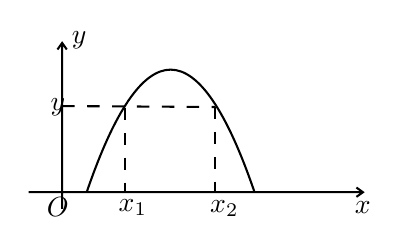
\begin{tikzpicture}[x=0.75pt,y=0.75pt,yscale=-1,xscale=1,scale=0.45]
            \draw  (50,212.81) -- (407.86,212.81)(85.79,53) -- (85.79,230.57) (400.86,207.81) -- (407.86,212.81) -- (400.86,217.81) (80.79,60) -- (85.79,53) -- (90.79,60)  ;
            \draw   (112,213) .. controls (171.95,37.76) and (231.9,37.76) .. (291.86,213) ;
            \draw  [dash pattern={on 4.5pt off 4.5pt}]  (85.86,120.57) -- (249.86,121.57) ;
            \draw  [dash pattern={on 4.5pt off 4.5pt}]  (152.86,122.57) -- (152.86,212.57) ;
            \draw  [dash pattern={on 4.5pt off 4.5pt}]  (249.86,121.57) -- (249.86,211.57) ;
            \draw (93,38) node [anchor=north west][inner sep=0.75pt]   [align=left] {$\displaystyle y$};
            \draw (143,217) node [anchor=north west][inner sep=0.75pt]   [align=left] {$\displaystyle x_{1}$};
            \draw (241,218) node [anchor=north west][inner sep=0.75pt]   [align=left] {$\displaystyle x_{2}$};
            \draw (396,220) node [anchor=north west][inner sep=0.75pt]   [align=left] {$\displaystyle x$};
            \draw (66,215) node [anchor=north west][inner sep=0.75pt]   [align=left] {$\displaystyle O$};
            \draw (70,109) node [anchor=north west][inner sep=0.75pt]   [align=left] {$\displaystyle y$};
        \end{tikzpicture}
    \end{center}
    所以\textbf{函数可以一对一,也可以多对一,统称为单值函数}.
    \begin{center}
        \tikzset{every picture/.style={line width=0.75pt}} %set default line width to 0.75pt        
        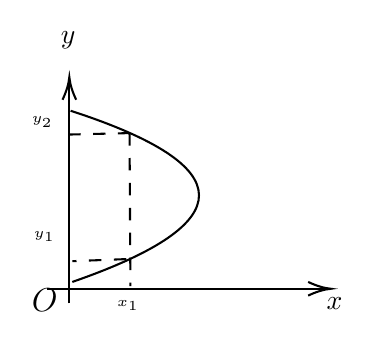
\begin{tikzpicture}[x=0.75pt,y=0.75pt,yscale=-1,xscale=1]
            %uncomment if require: \path (0,300); %set diagram left start at 0, and has height of 300

            %Straight Lines [id:da7957062642323978] 
            \draw    (220.57,170.29) -- (355.57,170.29) ;
            \draw [shift={(357.57,170.29)}, rotate = 180] [color={rgb, 255:red, 0; green, 0; blue, 0 }  ][line width=0.75]    (10.93,-3.29) .. controls (6.95,-1.4) and (3.31,-0.3) .. (0,0) .. controls (3.31,0.3) and (6.95,1.4) .. (10.93,3.29)   ;
            %Straight Lines [id:da31198976122474575] 
            \draw    (231.57,177.29) -- (231.57,70.29) ;
            \draw [shift={(231.57,68.29)}, rotate = 90] [color={rgb, 255:red, 0; green, 0; blue, 0 }  ][line width=0.75]    (10.93,-3.29) .. controls (6.95,-1.4) and (3.31,-0.3) .. (0,0) .. controls (3.31,0.3) and (6.95,1.4) .. (10.93,3.29)   ;
            %Straight Lines [id:da5655592463420158] 
            \draw  [dash pattern={on 4.5pt off 4.5pt}]  (260.57,95.29) -- (261,169) ;
            %Straight Lines [id:da8571495896140271] 
            \draw  [dash pattern={on 4.5pt off 4.5pt}]  (259,156) -- (233,157) ;
            %Straight Lines [id:da9798041145850536] 
            \draw  [dash pattern={on 4.5pt off 4.5pt}]  (231,96) -- (260.57,95.29) ;
            %Shape: Parabola [id:dp09151495358584594] 
            \draw   (233,167) .. controls (314.65,138.69) and (314.38,111.2) .. (232.18,84.52) ;
            % Text Node
            \draw (226,45) node [anchor=north west][inner sep=0.75pt]   [align=left] {$\displaystyle y$};
            % Text Node
            \draw (354,173) node [anchor=north west][inner sep=0.75pt]   [align=left] {$\displaystyle x$};
            % Text Node
            \draw (212,169) node [anchor=north west][inner sep=0.75pt]  [font=\large] [align=left] {$\displaystyle O$};
            % Text Node
            \draw (253.07,174.29) node [anchor=north west][inner sep=0.75pt]  [font=\tiny] [align=left] {$\displaystyle x_{1}$};
            % Text Node
            \draw (213,141) node [anchor=north west][inner sep=0.75pt]  [font=\tiny] [align=left] {$\displaystyle y_{1}$};
            % Text Node
            \draw (212,86) node [anchor=north west][inner sep=0.75pt]  [font=\tiny] [align=left] {$\displaystyle y_{2}$};
        \end{tikzpicture}
    \end{center}
    但是,如果一个$x$对应一个$y_1$,同时对应另一个$y_2$,也就是一对多,这叫做多值函数.(高等数学中研究对象主要是单值函数)\footnote{多值函数是不是函数取决于对于函数的定义。可以说狭义的函数特指单值函数,但是广义的函数既包含单值函数,也包含多值函数。}
\end{criterion}
\subsection{函数的表示}
\subsubsection{表格}
\begin{table}[H]
    \begin{center}
        \begin{tabular}{|l|l|l|l|l|l|l|}
            \hline
            $x$    & $ 1$ & $2$ & $3$ & $4$ & $5$  & $6$  \\ \hline
            $y=2x$ & $2$  & $4$ & $6$ & $8$ & $10$ & $12$ \\ \hline
        \end{tabular}
    \end{center}
\end{table}
\subsubsection{图像}
\begin{figure}[H]
    \centering 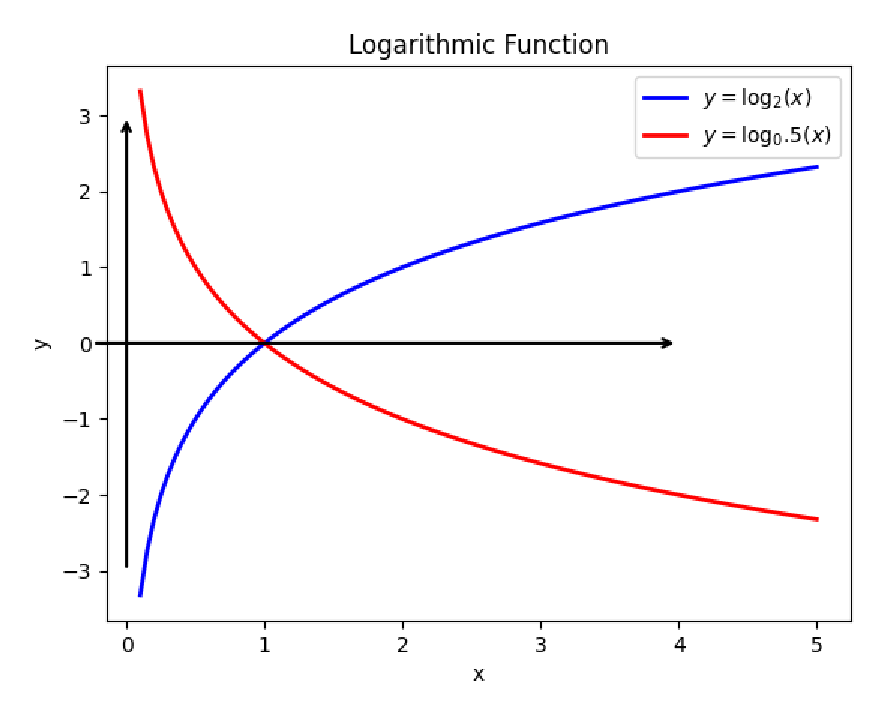
\includegraphics[width=
        0.6 \linewidth]{1.3.3.eps} \caption{对数函数图像}
\end{figure}
\subsubsection{解析式}
$$
    \boxed{y=2x}
$$